\section{KFAC: Block-diagonal inverse approx, $\breve{F}^{-1} \approx \tilde{F}^{-1}$}
\frame{\tableofcontents[currentsection, hideothersubsections]}

\begin{frame}
\frametitle{KFAC: Block-diagonal inverse approx, $\breve{F}^{-1} \approx \tilde{F}^{-1}$}
\begin{figure}
    \centering
    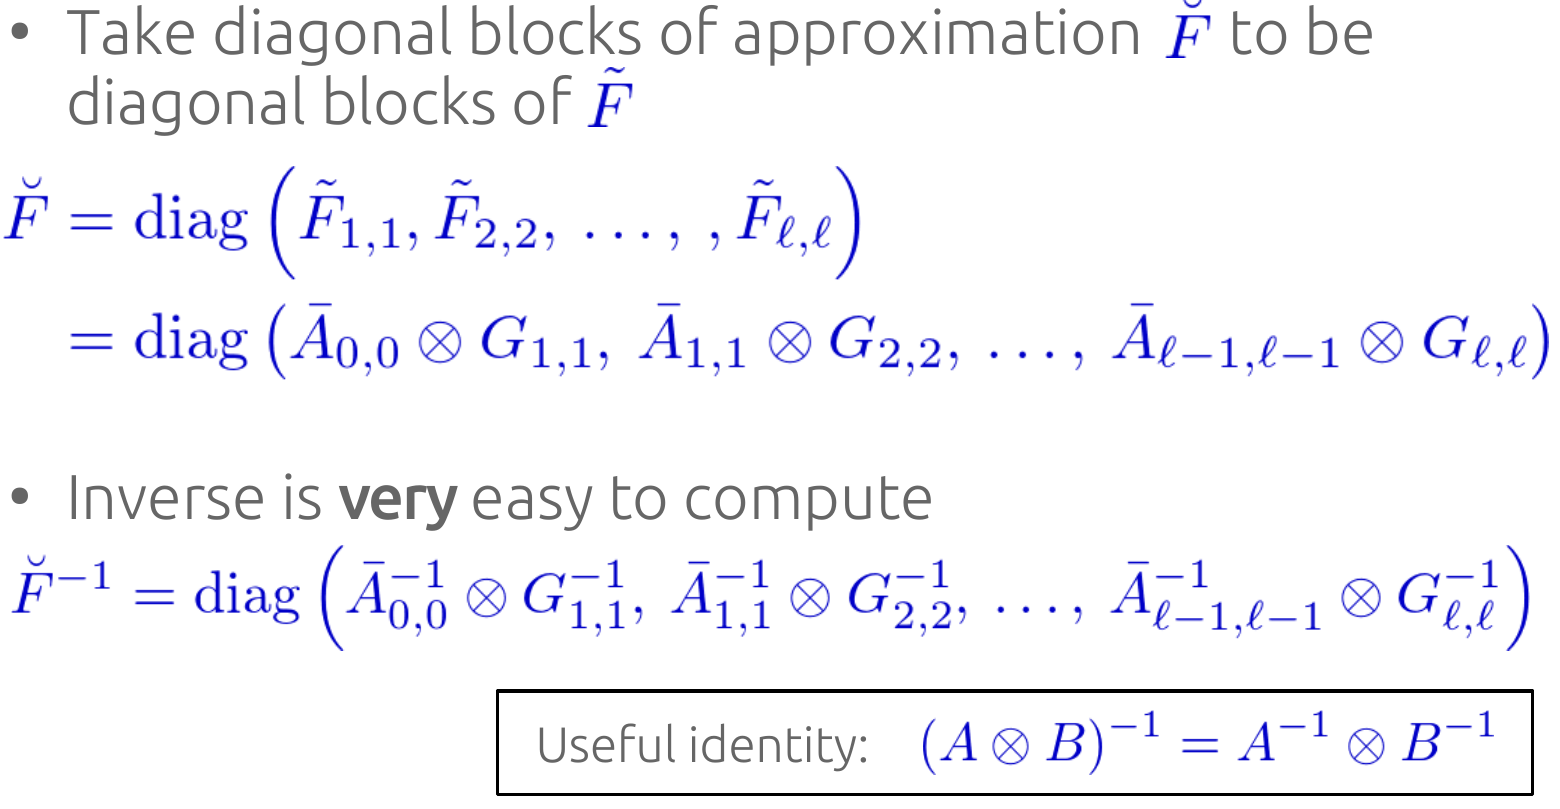
\includegraphics[scale=0.275]{kfac_08}
\end{figure}
NOTE: this is equivalent to approximating Fisher itself as block-diagonal
\end{frame}

\begin{frame}
\frametitle{KFAC: Block-diagonal inverse approx, $\breve{F}^{-1} \approx \tilde{F}^{-1}$}
\begin{figure}
    \centering
    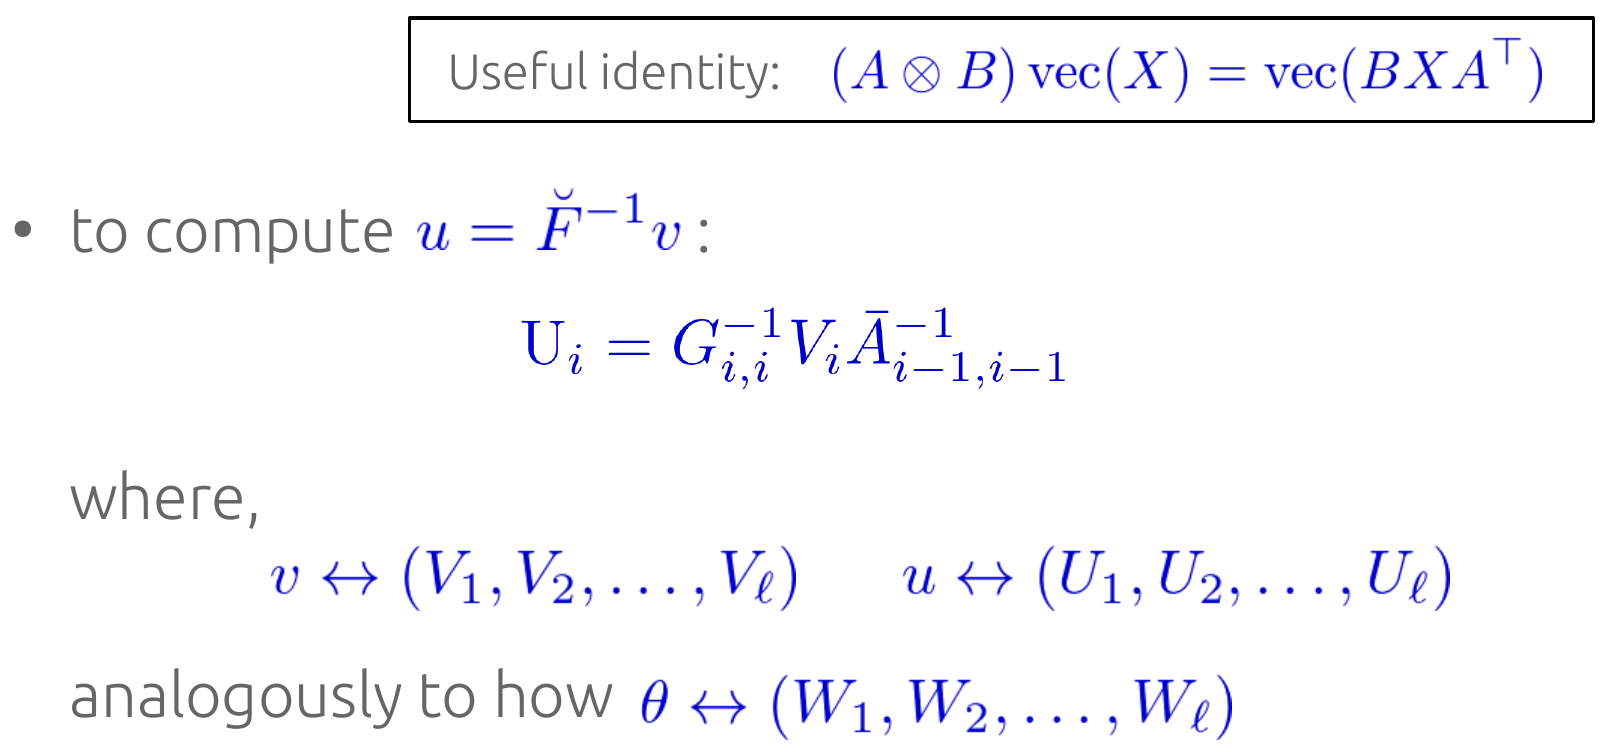
\includegraphics[scale=0.275]{kfac_09}
\end{figure}
\end{frame}

\begin{frame}
\frametitle{KFAC: Block-diagonal inverse approx, $\breve{F}^{-1} \approx \tilde{F}^{-1}$}
Left to right: \\
$\tilde{F}$, its approximations $\breve{F}$ (top) and $\hat{F}$ (bottom), their absolute difference

\begin{figure}
    \centering
    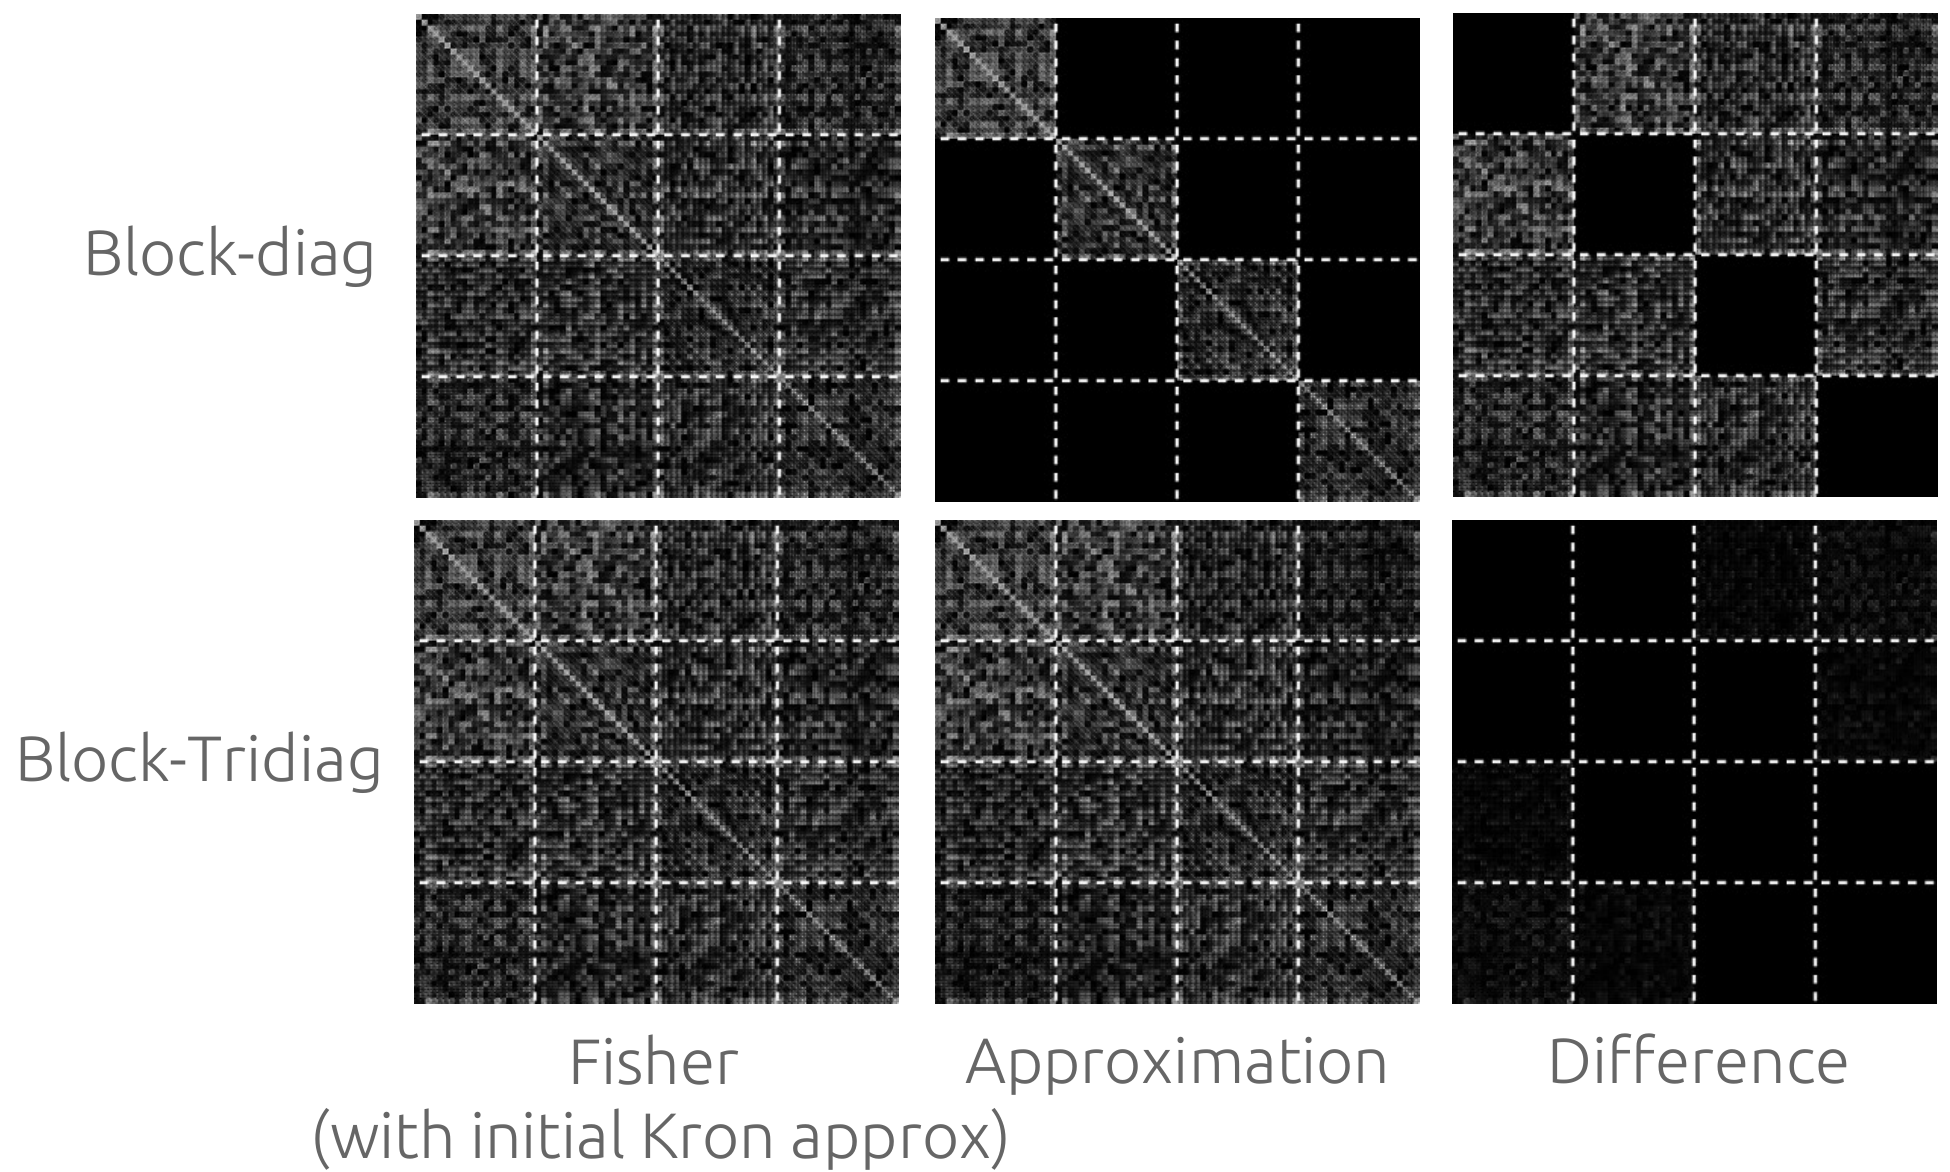
\includegraphics[scale=0.175]{kfac_10}
\end{figure}

\begin{itemize}
    \item the off-tridiagonal blocks of the bottom right matrix, while being very close to zero, are
    actually NON-zero (hard to see from the plot)
    % \item the plot is of the absolute values of the entries
\end{itemize}


\end{frame}
